\section{Introduzione}
In questa relazione gli autori descriveranno l'algoritmo di model-checking locale per aCTL. Dopo una breve introduzione dove verrano descritti i motivi della verifica formale del modello di un sistema, verranno descritti gli argomenti principali che serviranno per la descrizione dell'algoritmo di model-checking. Parleremo dei Label Transition System (LTS), in italiano sistema di transizione etichettato, utilizzati per la rappresentazione e la modellazione dei sistemi. Verrà definita la logica aCTL che permette di esprimere formalmente le proprietà che un sistema deve rispettare.
Infine verrà descritto l'algoritmo di model-checking locale. 
\\

%\textbf{Correttezza e completezza  Piccolo esempio da usare nella relazione per descrivere i concetti.}

\subsection{Importanza della correttezza del software}
Un programma si dice \emph{corretto} se il suo comportamento è conforme alle specifiche dei requisiti. In altre parole, possiamo dire che un software è corretto se fa esattamente quello per cui è stato creato.
L'importanza della correttezza del software diventa un concetto fondamentale soprattutto in ambiente considerato critico. Ad esempio: sistemi di controllo, impianti industriali, sistemi di trasporto, protocolli di comunicazione, etc\dots.

\begin{figure}[ht]
\begin{center}
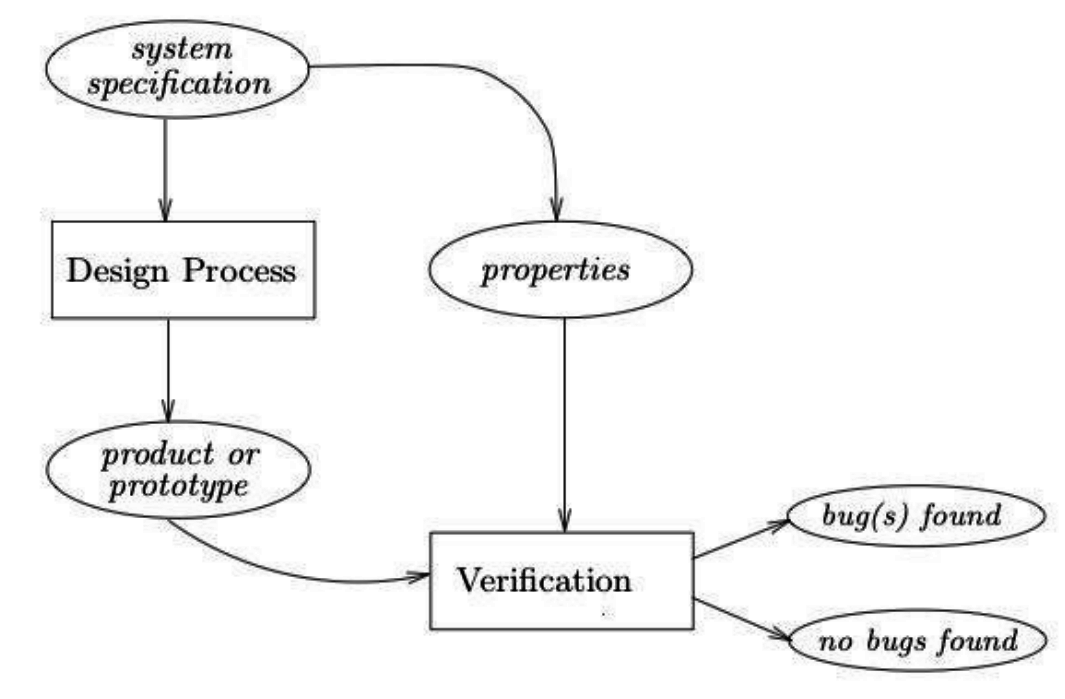
\includegraphics[scale=0.45]{img/Modello1.png}
\caption{Modello classico di ciclo di sviluppo del software.}
\label{fig:modello}
\end{center}
\end{figure}

In figura \ref{fig:modello} viene mostrato un approccio per la verifica di sistemi. Questo modello di ciclo di sviluppo del software presenta difetti importanti. La verifica del progetto viene fatta in fase avanzata dello sviluppo del codice. Modificare il codice sorgente nelle ultime fasi dello sviluppo potrebbe portare a numerosi problemi e rendere necessarie anche modifiche importanti. Inoltre, come mostrato in figura \ref{fig:costo_errori}, si può notare in quali fasi di sviluppo viene introdotto il maggior numero di errori e la loro incidenza sul loro costo di risoluzione. L'idea è quindi quella di trovare gli errori già nelle prime fasi del ciclo di sviluppo.

\begin{figure}[ht]
\begin{center}
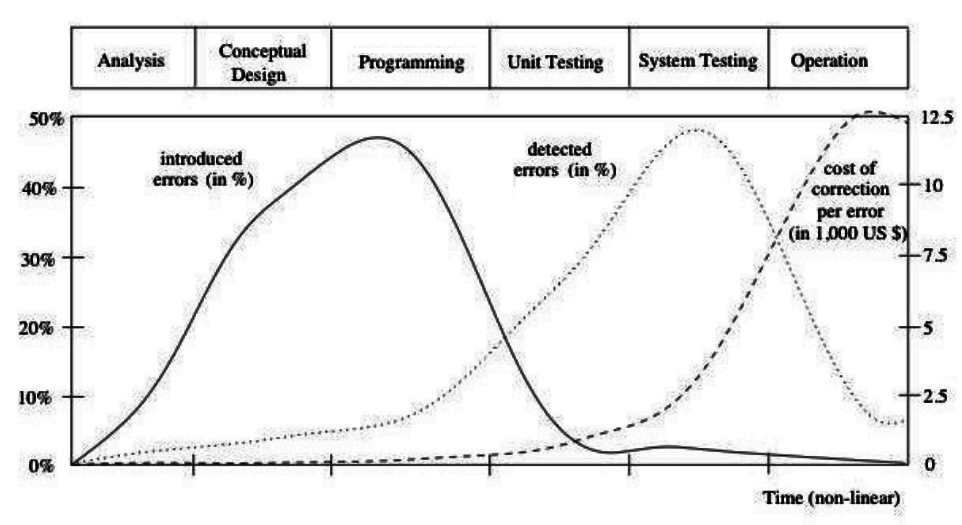
\includegraphics[scale=0.45]{img/costo_errori.png}
\caption{Grafico che mostra: introduzione degli errori, rilevazione degli errori e costo di correzione degli errori durante il ciclo di sviluppo del software.}
\label{fig:costo_errori}
\end{center}
\end{figure}